\section{Experiments and Results}
\label{sec:results}

We evaluate the MRANet model in four experiments, each probing a different
hypothesis about why local ML predictions might accelerate SCF convergence.
Training uses 51 molecules from the W4-11 dataset~\cite{karton2011w411}
(45 train, 3 validation, 3 test) at MADNESS production settings ($k=8$,
$\epsilon=10^{-6}$).

\subsection{Density Coefficient Prediction}
\label{sec:density_prediction}

Our first model used multi-task training with Kendall
uncertainty-weighted loss~\cite{kendall2018multitask} to jointly predict
density s-coefficients ($\rho_s$) and refinement labels. This produced a
train MSE ratio of 2.99$\times$ and validation ratio of 2.84$\times$
relative to the $\rho_0$ baseline, meaning the model performed nearly
three times \emph{worse} than simply copying the promolecular density.
Inspection of the learned uncertainty parameters revealed the cause:
$\sigma_{\rho_s}$ grew without bound during training, progressively
zeroing the $\rho_s$ gradient while the classification head consumed
the entire learning signal.

Single-task ablation (removing the refinement head entirely) resolved
this interference. The single-task model achieved a train ratio of
1.006$\times$ and validation ratio of 1.004$\times$, reaching approximate
parity with $\rho_0$.

Per-level MSE analysis on the validation molecules (ethanol, SO$_2$,
HN$_3$) exposed a more informative pattern
(\autoref{fig:per_level_mse}).

\begin{figure}[htbp]
  \centering
  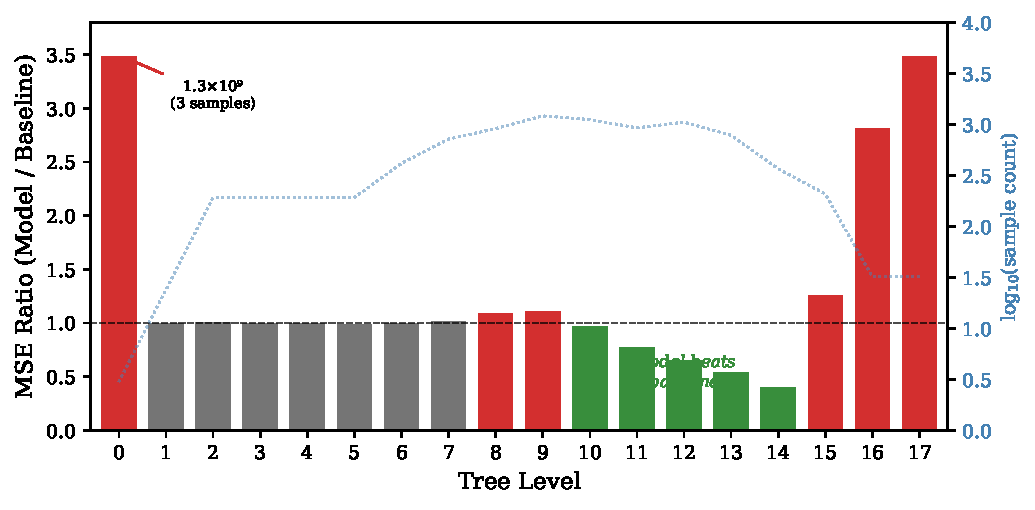
\includegraphics[width=\columnwidth]{figures/fig2_per_level_mse.pdf}
  \caption{Per-level MSE ratio (model/baseline) on the validation set. The model beats $\rho_0$ at levels 10--14 (ratio $< 1$) but matches or slightly exceeds it at coarse levels 1--9 (ratio $\geq 1$). Levels 0, 15--17 have too few training samples for reliable prediction.}
  \label{fig:per_level_mse}
\end{figure}

After applying level-aware masking (hard
cutoff below 200 training samples, $\sqrt{n/n_\text{max}}$ sample
weighting), the model beat $\rho_0$ at fine levels and matched it at
coarse levels:
%
\begin{itemize}
  \item Level 0 (3 samples): $1.34 \times 10^{9}\times$ baseline.
        Catastrophic failure from extreme data scarcity, masked during
        training but exposed at inference.
  \item Levels 1--9 (24--1216 samples): $1.00$--$1.12\times$.
        Near-parity with $\rho_0$.
  \item Level 10 (1120 samples): $0.98\times$.
  \item Level 11 (928 samples): $0.79\times$.
  \item Level 12 (1056 samples): $0.67\times$.
  \item Level 13 (784 samples): $0.55\times$.
  \item Level 14 (368 samples): $0.41\times$.
  \item Level 15 (208 samples): $1.27\times$.
        Performance degrades as sample counts drop below the masking
        threshold.
  \item Levels 16--17 (32 samples each): $2.83\times$ and $5.34\times$.
\end{itemize}
%
The model learns a genuine correction to $\rho_0$ at levels 10--14,
where training data is abundant and the density correction signal is
spatially localized near nuclei. At coarser levels, the correction
is a non-local function of electron-electron interactions that cannot
be inferred from same-level halo features alone.

We constructed a level-clamped predictor that uses the ML model at
levels 10--14 and falls back to $\rho_0$ elsewhere. This hybrid
achieved an aggregate validation MSE of $0.97\times$ baseline: a 3\%
improvement over $\rho_0$. The natural question is whether this
improvement translates to fewer SCF iterations.

\subsection{Parent Node Features}
\label{sec:parent_features}

One hypothesis for the coarse-level plateau is that the model lacks
multi-resolution context. To test this, we concatenated parent-node
$\rho_0$ and $V_\text{nuc}$ s-coefficients (1024 additional floats per
sample) to the trunk input, increasing it from 1792 to 2816 dimensions
and total parameters from 3.0M to 4.1M. Because the first layer shape
changed, we trained from scratch rather than fine-tuning.

The result was negative. Per-level MSE ratios were identical to those
of the model without parent features, within training noise. The parent
$\rho_0$ and $V_\text{nuc}$ encode the same atomic superposition signal
at coarser resolution. They do not contain the density correction
(exchange-correlation, orbital relaxation, bonding redistribution)
because that correction is what the converged SCF procedure computes.
Adding a coarser copy of the input does not introduce new information
about the target.

\subsection{SCF Convergence Test}
\label{sec:scf_test}

We injected the level-clamped density into MADNESS and ran full SCF
calculations on 7 molecules at two convergence thresholds ($10^{-6}$
and $10^{-8}$), yielding 14 comparisons against the $\rho_0$ baseline
(\autoref{tab:scf_iterations}).

\begin{table}[htbp]
\centering
\caption{SCF iteration counts for level-clamped ML density (levels 10--14) vs.\ promolecular baseline ($\rho_0$). All 14 comparisons yield identical iteration counts. Ground-state energies agree to 8+ significant figures.}
\label{tab:scf_iterations}
\begin{tabular}{lccrrc}
\toprule
Molecule & $N_e$ & Thresh & Baseline & ML & $E_\text{base}$ (Ha) \\
\midrule
CH$_3$OH & 18 & $10^{-6}$ & 12 & 12 & -114.85038034 \\
CH$_3$OH & 18 & $10^{-8}$ & 12 & 12 & -114.85038034 \\
Ethanol & 26 & $10^{-6}$ & 12 & 12 & -153.81559584 \\
Ethanol & 26 & $10^{-8}$ & 12 & 12 & -153.81559584 \\
SO$_2$ & 32 & $10^{-6}$ & 14 & 14 & -546.34469275 \\
SO$_2$ & 32 & $10^{-8}$ & 14 & 14 & -546.34469265 \\
HN$_3$ & 22 & $10^{-6}$ & 13 & 13 & -163.57199524 \\
HN$_3$ & 22 & $10^{-8}$ & 13 & 13 & -163.57199524 \\
H$_2$O$_2$ & 18 & $10^{-6}$ & 12 & 12 & -150.55376660 \\
H$_2$O$_2$ & 18 & $10^{-8}$ & 12 & 12 & -150.55376660 \\
C$_2$H$_2$ & 14 & $10^{-6}$ & 10 & 10 & -76.63064903 \\
C$_2$H$_2$ & 14 & $10^{-8}$ & 10 & 10 & -76.63064903 \\
Glyoxal & 30 & $10^{-6}$ & 13 & 13 & -226.15979738 \\
Glyoxal & 30 & $10^{-8}$ & 13 & 13 & -226.15979738 \\
\bottomrule
\end{tabular}
\end{table}


All 14 comparisons produced identical iteration counts. CH$_3$OH
converged in 12 iterations with both initial guesses. Ethanol: 12.
SO$_2$: 14. HN$_3$: 13. H$_2$O$_2$: 12. C$_2$H$_2$: 10.
Glyoxal: 13. Ground-state energies agreed to 8 or more significant
figures (e.g., $E_{\text{CH}_3\text{OH}} = -114.85038034$ Ha for the
baseline vs.\ $-114.85038032$ Ha for the ML density). The correct
electronic state was recovered in every case.

The mechanism is straightforward. MADNESS uses a multi-protocol SCF
strategy: the first protocol solves at a coarse threshold
($\epsilon = 10^{-4}$), and subsequent protocols refine progressively.
The coarse protocol sets the density at levels 1--9, which determines
the convergence path. Fine-level improvements at levels 10--14, where
the ML model outperforms $\rho_0$, are projected away when the tree is
compressed to the coarse threshold. By the time later protocols operate
at fine resolution, the density has already been updated by SCF
iterations and the initial guess is irrelevant.

Tightening the final threshold from $10^{-6}$ to $10^{-8}$ does not
change this conclusion. The additional refinement occurs at even finer
levels, but the coarse-level convergence path remains identical.

\subsection{Tree Structure Prediction}
\label{sec:tree_prediction}

The density prediction results suggest that the local receptive field
limits regression accuracy at coarse levels. We tested whether the same
limitation applies to a simpler task: predicting which nodes require
adaptive refinement (a binary classification problem).

Multi-task training (density regression + refinement classification)
achieved F1 = 0.857. The learned $\sigma_{\rho_s}$ shrank to 0.075,
upweighting the density loss by 89$\times$ and starving the refinement
classification head. Training the refinement head alone with focal
loss~\cite{lin2017focal} ($\gamma = 2$, $\alpha = 0.75$) yielded
F1 = 0.860, a delta of 0.003. Removing multi-task interference had
negligible effect on the classification ceiling.

We tested the refine-only model in an SCF tree-walk: starting from
the ML-predicted tree structure rather than the $\rho_0$ tree.
CH$_3$OH required 31 iterations compared to 12 with the baseline
tree, a factor of 2.6$\times$ worse. The model did recover the
correct electronic state (energies agreed to 7 significant figures:
$-114.85038034$ vs.\ $-114.85037863$ Ha), confirming that the SCF
procedure corrects the tree errors at the cost of additional
iterations.

The classification task faces the same receptive field limitation
as regression. Whether a node at level $N$ should be refined depends
on the density structure at levels 0 through $N-1$, which determines
the wavelet coefficients that trigger refinement in MADNESS. A model
restricted to same-level halo neighbors cannot access this information.
